
\begin{subsection}{Clustering from Different Point of View}

We worked on three different methods for clustering, all based on similarity measures.
They share the idea of creating a similarity graph $G$ (potentially complete) in which each vertice $V$ represents an images for one point of interest, and
each edge $E$ represents the similarity between two images accoring to a similarity metric $M$ based on a set of features $F$.
Figure~\ref{fig:bigben} shows a small sample based on 4 images of Big Ben.
Next, we are going to expain each algorithm and how we combined them.

\begin{figure}[h!]
\centering
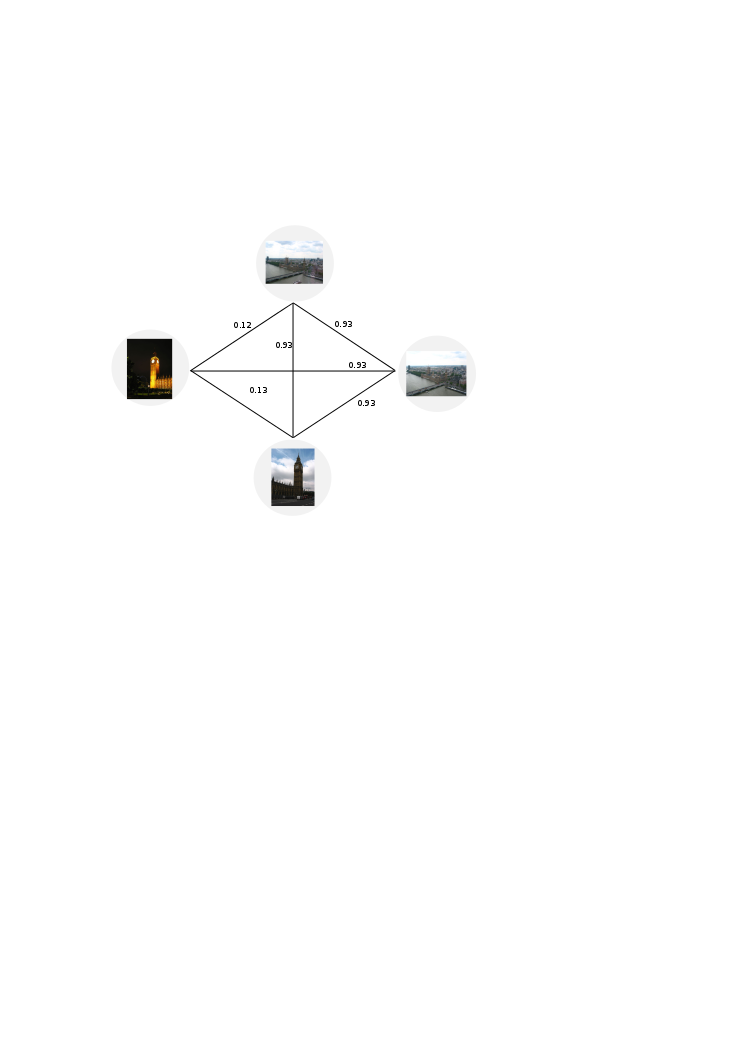
\includegraphics[width=0.2\textwidth]{figs/bigben}

\caption{This figure is terrible...I will improve it soon}
\label{fig:bigben}
\end{figure}

\begin{subsubsection}{Metis}

%The best way for partitioning $G$ is NP-hard...
The first approach, called Metis~\cite{metis},
tries to collapse similar and neighbor nodes, reducing the initial graph to a smaller one (known as coarsening step).
Then, it divides the coarsest graph into a pre-defined number of graphs, generating the clusters that we use.  

\end{subsubsection}

\begin{subsubsection}{Spectral}

Spectral clustering~\cite{spectral} can also be seen as a graph partitioning method, which measures both the total dissimilarity between the different groups 
as well as the total similarity within the groups. We used the Scikit-learn\footnote{\url{http://scikit-learn.org/stable/modules/generated/sklearn.cluster.SpectralClustering.html#sklearn.cluster.SpectralClustering}} of this method. 

\end{subsubsection}

\begin{subsubsection}{Hierarchical}
Hierarchical clustering~\cite{hierarchical} is based on the idea of a hierarchy of clusters. A tree is build in which the root gathers all the samples and the leaves are clusters with only one sample. This tree can be built bottom-up or top down. We used the bottom-up implementation from Scikit-learn\footnote{\url{http://scikit-learn.org/stable/modules/generated/sklearn.cluster.AgglomerativeClustering.html#sklearn.cluster.AgglomerativeClustering}}.

\end{subsubsection}

\begin{subsubsection}{Merging}

After applying different clustering methods on the whole 2013 and 2014 development set, 
we reached the conclusion that it is acctually difficult to say which method would work best at 2014 testset.
Therefore, we decide to come up with a merging algorithm, which should take into account different point of views from each clustering methods used,
and potentially would be more robust than using one single clustering algorithm.

Our merging procedure provides a re-rank of an initial ranked list. Starting from one pivot document (in this case, the top ranked in the original list), 
it iterates over the original list, including new documents that are not frequently assigned to the same cluster of any other already included document. 
Algorithm~\ref{alg:merge} shows the algorithm in more details.


\renewcommand{\algorithmicrequire}{\textbf{Input:}}
\renewcommand{\algorithmicensure}{\textbf{Output:}}
\newcommand{\algorithmicbreak}{\textbf{break}}
\newcommand{\Break}{\State \algorithmicbreak}
\algrenewcommand\Return{\State \algorithmicreturn{} }%
%\def\BState{\State\hskip-\ALG@thistlm}
\begin{algorithm}
\caption{Merging of different clustering methods}
\label{alg:merge}
\begin{algorithmic}[1]
\Require L, F, min, mean, max, min\_increment, mean\_increment, max\_increment
\Ensure FinalList 

\Procedure{Merge}{}
\State $\text{FinalList} \gets \text{[ ]}$
\State $\textit{pivot} \gets \text{L.pop()}$
\State $\text{finalList.push(pivot)}$
\While{L.hasElement()}
\State $\textit{e} \gets \text{L.pop()}$
\State $\text{include} \gets \text{True}$

\State $\text{TempList} \gets \text{[ ]}$
\ForAll {Element $ie$ in finalList}
\State $\text{TempList} \gets \text{F[e][ie]}$
\EndFor

\If {max(TempList) > maxvalue} 
\State $\text{include} \gets \text{False}$
\Break
\EndIf
\If {min(TempList) > minvalue} 
\State $\text{include} \gets \text{False}$
\Break
\EndIf
\If {mean(TempList) > meanvalue} 
\State $\text{include} \gets \text{False}$
\Break
\EndIf
\If {include} 
\State $\text{finalList.push(ie)}$
\Else
\State $\text{L.push(ie)}$
\EndIf
\State $\text{min} \gets \text{min} + \text{min\_increment}$
\State $\text{max} \gets \text{max} + \text{max\_increment}$
\State $\text{mean} \gets \text{mean} + \text{mean\_increment}$
\EndWhile
\Return finalList
\EndProcedure
\end{algorithmic}
\end{algorithm}

\end{subsubsection}

\end{subsection}



